\section{Results}
\label{sec:results}

We first evaluate strand reconstruction on synthetic scenes
(Section~\ref{sec:res-density}), then examine depth ordering
(Section~\ref{sec:res-depth}) and application to real SEM images
(Section~\ref{sec:res-real}). Component ablations
(Section~\ref{sec:res-ablation}) and comparisons with published methods
(Section~\ref{sec:res-comparators}) assess the contributions and performance
of the reconstruction method.

\subsection{Reconstruction on synthetic images}
\label{sec:res-density}

Across the \PlectaHeldoutSceneCount{} synthetic scenes, PLECTA
achieved a mean common-fragment pairwise \Fone{} of
\PlectaHeldoutFOneMean{} (95\% bootstrap CI
[\PlectaHeldoutFOneCILow{}, \PlectaHeldoutFOneCIHigh{}]).
Table~\ref{tab:plecta-heldout} summarises reconstruction scores overall and by
areal coverage.

\begin{table}[tbp]
    \centering
    \caption{Held-out reconstruction scores overall and by target areal
    coverage. VI denotes variation of information, for which lower is better;
    higher is better for the other metrics.}
    \label{tab:plecta-heldout}
    \small
    % Generated by scripts/results/make_plecta_results.py; do not edit.
\begin{tabular}{lrrrrrrrr}
\toprule
Group & $n$ & $F_1$ & Precision & Recall & ARI & VI split & VI merge & VI total \\
\midrule
All & 128 & 0.85 & 0.87 & 0.84 & 0.85 & 0.26 & 0.22 & 0.47 \\
20\% & 32 & 0.91 & 0.93 & 0.90 & 0.91 & 0.14 & 0.09 & 0.23 \\
30\% & 32 & 0.87 & 0.89 & 0.86 & 0.87 & 0.21 & 0.16 & 0.37 \\
40\% & 32 & 0.86 & 0.86 & 0.85 & 0.85 & 0.24 & 0.22 & 0.47 \\
60\% & 32 & 0.77 & 0.79 & 0.76 & 0.77 & 0.44 & 0.39 & 0.82 \\
\bottomrule
\end{tabular}

\end{table}

Performance decreased with scene density: mean \Fone{} fell from
\PlectaDensityTwoZeroFOneMean{}
[\PlectaDensityTwoZeroFOneCILow{}, \PlectaDensityTwoZeroFOneCIHigh{}] at 20\%
coverage to \PlectaDensitySixZeroFOneMean{}
[\PlectaDensitySixZeroFOneCILow{}, \PlectaDensitySixZeroFOneCIHigh{}] at 60\%,
monotonically through the intermediate strata.
Per-scene runtime had median \PlectaHeldoutRuntimeMedian{}~s, ranging to
\PlectaHeldoutRuntimeMaximum{}~s on the densest scenes;
Section~\ref{sec:res-comparators} measures cost systematically.

PLECTA operates on the strand-axis mask, so reconstruction difficulty depends
on centreline density and geometry rather than areal coverage alone. The same
areal coverage can arise from a different centreline density under another
bundle-width distribution and may therefore produce different reconstruction
performance. Within the fixed $512\times512$-pixel frame and 7--16-pixel
bundle-width range used here, areal coverage provides a consistent within-study
stratification.

\label{sec:res-mask}%
To assess sensitivity to gaps and raster irregularities, we compared
reconstruction from clean and degraded masks of the same scenes. Across the
\PlectaRobustnessSceneCount{} synthetic scenes,
mean \Fone{} was \PlectaRobustnessDegradedFOneMean{} from degraded axes and
\PlectaRobustnessCleanFOneMean{} from the corresponding clean axes. The paired
clean-minus-degraded change was \PlectaCleanMinusDegradedFOneMean{} (95\% CI
[\PlectaCleanMinusDegradedFOneCILow{},
\PlectaCleanMinusDegradedFOneCIHigh{}]). Modelled gaps and raster
irregularities therefore caused a small reduction in reconstruction accuracy
under this generator. The difference was greatest at low coverage and narrowed
at 50--60\,\%, consistent with junction ambiguity becoming more influential
at higher density.

Figure~\ref{fig:examples} shows representative reconstructions at three
coverage levels, selected by proximity to the median \Fone{} of each stratum.

\begin{figure}[tbp]
    \centering
    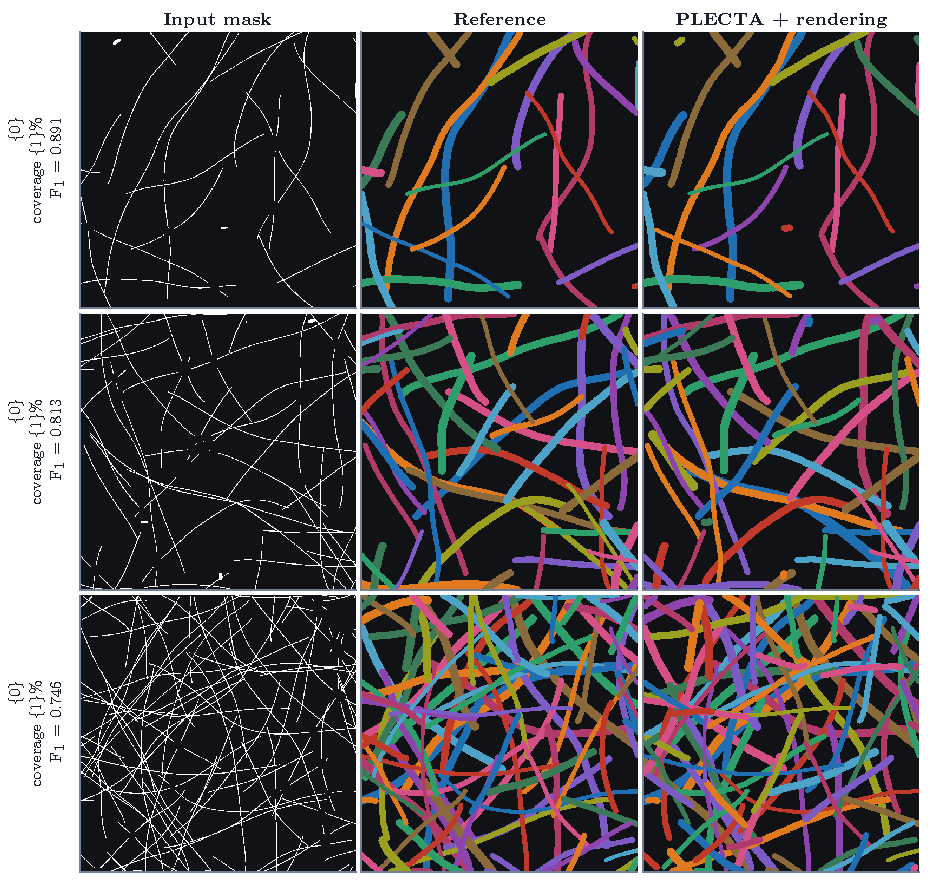
\includegraphics[width=\linewidth]{figures/fig_plecta_examples.pdf}
    \caption{Reconstruction at three coverage levels, each the scene closest
    to the median \Fone{} of its stratum, shown as a horizontal window of the
    scene. Columns: the degraded input mask, the overlap-aware reference, and
    PLECTA's strands at their fitted widths. The score beside each row is the
    grouping's, not the rendering's. Strand colours are arbitrary and not
    matched between columns.}
    \label{fig:examples}
\end{figure}

\subsection{Depth decomposition}
\label{sec:res-depth}

The stages above reconstruct strands in projection but do not establish which
strand lies above at a crossing. After grouping is fixed, the depth stage uses
the greyscale image to assess the continuity of each strand's brightness across
the crossing relative to local noise. It reconciles these local estimates into
a globally consistent vertical order and assigns non-interpenetrating heights.

The stage was evaluated on \PlectaDepthSceneCount{} depth-resolved scenes from
Section~\ref{sec:mm-synth}, at two areal coverages and under two input
conditions. Reference 2-D geometry isolates the depth decision, whereas binary
axis masks include reconstruction error. Table~\ref{tab:depth-order} reports
both using the measures defined in \suppdepth{}. Its crossing rows score local
over/under decisions before reconciliation, once for every crossing; its
stacking rows score the final order, once for every pair of strands.

\begin{table}[!ht]
\centering
\caption{The depth stage on \PlectaDepthSceneCount{} synthetic scenes whose
true vertical order is known. Chance is \PlectaDepthChance{} for every
accuracy shown.}
\label{tab:depth-order}
\begin{tabular}{lcccc}
\toprule
& \multicolumn{2}{c}{Given 2-D geometry} & \multicolumn{2}{c}{Reconstructed 2-D} \\
\cmidrule(lr){2-3}\cmidrule(lr){4-5}
Areal coverage & 20\,\% & 40\,\% & 20\,\% & 40\,\% \\
\midrule
Projected crossings per scene & 28 & 150 & 28 & 150 \\
Crossings recovered & 1.000 & 1.000 & 0.857 & 0.746 \\
Order accuracy, all crossings & 0.815 & 0.744 & 0.729 & 0.556 \\
Order accuracy, decided only & 0.890 & 0.885 & 0.961 & 0.906 \\
Abstained & 0.085 & 0.161 & 0.117 & 0.179 \\
Depth order, crossing pairs & 0.863 & 0.856 & 0.915 & 0.852 \\
Depth order, all pairs & 0.671 & 0.708 & 0.703 & 0.715 \\
Instance pairs sharing a component & 0.392 & 0.842 & 0.361 & 0.746 \\
Layer agreement & 0.656 & 0.418 & 0.702 & 0.382 \\
\bottomrule
\end{tabular}

\end{table}

Among crossings for which an order was assigned, accuracy ranged from
\PlectaDepthDecidedLow{} to \PlectaDepthDecidedHigh{} across both input
conditions and densities. The all-crossing scores were lower
(\PlectaDepthAllLow{}--\PlectaDepthAllHigh{}) because they include crossings
the 2-D stage did not recover and those for which the depth stage abstained.
The table reports recovery and abstention rates alongside these scores.

Global order is limited to evidence that can travel through the crossing graph.
Only \PlectaDepthWithinLow{} to \PlectaDepthWithinHigh{} of strand pairs lie
within the same connected component, so the relative order of the remaining
pairs is not identifiable from the available crossing evidence. All-pair order
accuracy was consequently 0.67--0.72, compared with 0.85--0.91 for pairs that
cross. Layer agreement likewise fell from \PlectaDepthCleanCovTwoZeroLayers{}
to \PlectaDepthCleanCovFourZeroLayers{} as coverage doubled, although the
recovered number of layers remained close to the reference.

Figure~\ref{fig:resem-synth} shows what the stage produces on one synthetic
scene, from the binary axis mask through to the film the reconstruction
implies; Figure~\ref{fig:resem-real} is the same sequence on a real CNT SEM
field, which no depth ground truth can score.

\begin{figure}[!ht]
\centering
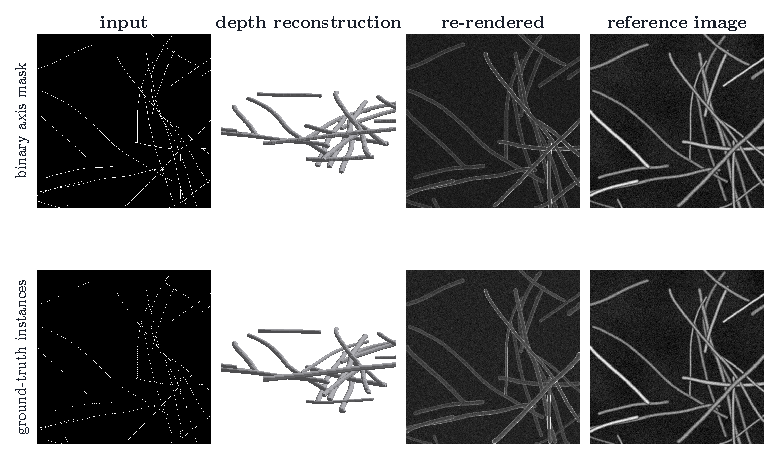
\includegraphics[width=\linewidth]{figures/fig_resem_synth.pdf}
\caption{Depth reconstruction of a synthetic scene from its binary axis mask.
The panels show the rendered greyscale image, a forward-model re-rendering from
the reconstructed depths and radii, and the inferred strand stack. The
re-rendering is a visual consistency check, not a scored quantity. The scene is
512\,px across in the generator's pixel units.}
\label{fig:resem-synth}
\end{figure}

\begin{figure}[tbp]
\centering
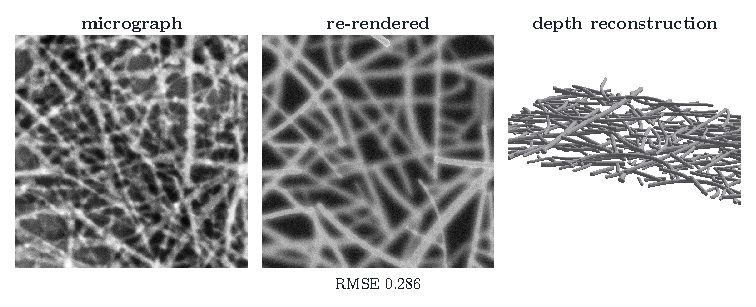
\includegraphics[width=\linewidth]{figures/fig_resem_real.pdf}
\caption{The same comparison on a real CNT SEM field, reconstructed from the
reference axis mask. The crop is 512\,px across, about 0.55\,\um{} of field
B58\_100. Real SEM provides no depth ground truth, so the depth order is shown
qualitatively; the forward-model appearance parameters are fitted to this
micrograph.}
\label{fig:resem-real}
\end{figure}

\subsection{Reconstruction on CNT SEM images}
\label{sec:res-real}
\label{sec:res-qualitative}

An upstream segmenter produces the binary strand-axis mask from each SEM
micrograph (Figure~\ref{fig:pipeline-upstream}), and PLECTA uses that mask
alone.

\begin{figure}[!ht]
    \centering
    % ---------------------------------------------------------------------------
%  Figure of Section 4.3.  Drawn in TikZ, in the document's own face at the
%  document's own size, replacing the matplotlib
%  figures/fig_pipeline_upstream.pdf whose generator now writes to
%  figures/archive/.
%
%  The upstream route is grey and the evaluated stage is not, which carries
%  the "not a contribution of this paper" distinction with line colour rather
%  than a filled region.  The training and inference clauses of the old
%  drawing live in the caption.
%
%  Requires the pk vocabulary defined in main.tex's preamble.
% ---------------------------------------------------------------------------
\begin{tikzpicture}[pk, x=1mm, y=1mm]

  % ---- training: the pair is manufactured --------------------------------
  \node[ext=32mm] (pmask)   at ( 30,   0) {Procedural\\binary mask};
  \node[ext=24mm] (gan)     at ( 79.5, 0) {CycleGAN};
  \node[ext=32mm] (semlike) at (129,   0) {SEM-like\\micrograph};

  \draw[flowsoft] (pmask) -- (gan);
  \draw[flowsoft] (gan)   -- (semlike);

  \node[ext=54mm] (corpus) at (79.5, -18)
    {Paired corpus: the procedural mask\\serves as the training label};

  \draw[flowsoft] (pmask.south)   |- (corpus.west);
  \draw[flowsoft] (semlike.south) |- (corpus.east);

  % ---- inference: the segmenter never sees an annotation -----------------
  \node[ext=32mm] (sem)    at ( 30,  -38) {Real SEM\\micrograph};
  \node[ext=24mm] (nnunet) at ( 79.5,-38) {Trained\\nnU-Net};
  \node[io=32mm]  (bmask)  at (129,  -38) {Binary strand-\\axis mask};

  \draw[flowsoft] (sem)    -- (nnunet);
  \draw[flowsoft] (nnunet) -- (bmask);
  \draw[flowsoft] (corpus.south) -- (nnunet.north);
  \node[note, anchor=west] at (82.5, -28.5) {trains};

  % ---- the stage this paper evaluates ------------------------------------
  \node[stage=32mm] (plecta) at (129, -56) {PLECTA};
  \draw[flow] (bmask) -- (plecta);

  \begin{scope}[on background layer]
    \node[scope, fit=(plecta)] (core) {};
  \end{scope}
  \node[scopelab, anchor=east, align=right] at (105, -56)
    {evaluated in this paper:\\reads that mask and nothing else};

  % ---- row labels, in the margin ------------------------------------------
  \node[note, anchor=south west] at (2,   8) {\textsc{training}};
  \node[note, anchor=south west] at (2, -31) {\textsc{inference}};

\end{tikzpicture}

    \caption{Upstream generation of the binary strand-axis mask. The segmenter
    is trained on procedurally generated image--mask pairs and requires no
    manual annotations for training or inference. Only the PLECTA stages inside
    the dashed boundary are evaluated here; the segmenter has its own
    evaluation \citep{ruehle2021workflow}.}
    \label{fig:pipeline-upstream}
\end{figure}

We evaluated \PlectaRealFieldCountLower{} manually annotated CNT-sheet fields
under two input conditions: the skeleton of the reference annotation and the
automatic nnU-Net axis \citep{ruehle2021workflow}. Both were scored against
the reference annotation, so the conditions differ only in the input mask. The
reference-derived axis tests grouping from curated real-image geometry; the
automatic axis evaluates the complete image-to-reconstruction workflow.
Figure~\ref{fig:real-sem} shows both conditions on one whole field.

\begin{figure}[tbp]
    \centering
    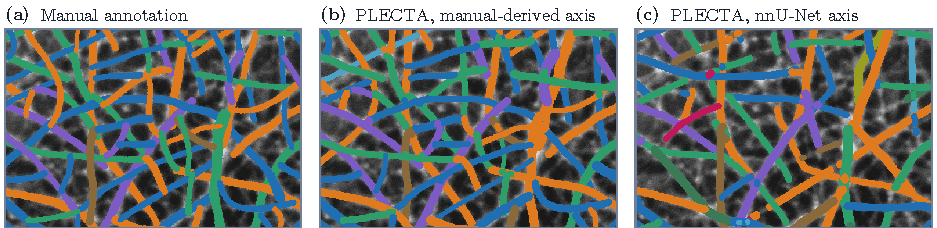
\includegraphics[width=\linewidth]{figures/fig_real_sem.pdf}
    \caption{Reconstruction of the whole B58\_110 field from two input-mask
    sources; the scale bar in (a) is 500\,nm. \textbf{(a)}~Reference
    annotation; \textbf{(b)}~reference-derived axis; \textbf{(c)}~PLECTA from
    that axis; \textbf{(d)}~automatic axis; and \textbf{(e)}~PLECTA from that
    axis with the same parameters. Input axes are dilated by one pixel for
    legibility. Predicted strands take the colour of their matched reference
    strand; crimson indicates no match.}
    \label{fig:real-sem}
\end{figure}

\begin{table}[tbp]
    \centering
    \caption{Reconstruction from reference-derived and automatic axes in three
    CNT SEM fields. Coverage is the fraction of the frame covered by full-width
    reference strands. Metrics are defined in Section~\ref{sec:mm-metrics};
    detection \Fone{} uses IoU \PlectaDetectionIoU{} and tolerance
    \PlectaPlacementTolerance{}\,px.}
    \label{tab:plecta-real-masks}
    \footnotesize
    % Generated by scripts/results/make_plecta_results.py; do not edit.
\begin{tabular}{lrllrrr}
\toprule
Field & Coverage & Input axis & Method & $F_1$ & Join $F_1$ & Det.\ $F_1$ \\
\midrule
B58\_100 & 44.0\,\% & Manual-derived & PLECTA & 0.89 & 0.93 & 0.94 \\
 &  &  & SIFNE & 0.89 & 0.92 & 0.92 \\
 &  &  & Basu$^{*}$ & 0.81 & 0.89 & 0.87 \\
 &  & U-Net & PLECTA & 0.46 & 0.56 & 0.63 \\
\addlinespace
B58\_110 & 46.7\,\% & Manual-derived & PLECTA & 0.84 & 0.91 & 0.93 \\
 &  &  & SIFNE & 0.81 & 0.89 & 0.92 \\
 &  &  & Basu$^{*}$ & 0.71 & 0.85 & 0.85 \\
 &  & U-Net & PLECTA & 0.45 & 0.59 & 0.60 \\
\addlinespace
B58\_300 & 41.5\,\% & Manual-derived & PLECTA & 0.95 & 0.96 & 0.96 \\
 &  &  & SIFNE & 0.90 & 0.94 & 0.93 \\
 &  &  & Basu$^{*}$ & 0.75 & 0.91 & 0.89 \\
 &  & U-Net & PLECTA & 0.47 & 0.62 & 0.58 \\
\bottomrule
\end{tabular}

\end{table}

Table~\ref{tab:plecta-real-masks} reports each field and condition. Mean
\Fone{} was \PlectaRealManualFOneMean{} from the reference-derived axis and
\PlectaRealUNetFOneMean{} from the automatic axis. The reference-derived
result establishes grouping on axes from real micrographs; the automatic
result measures sensitivity to the input mask. With only
\PlectaRealFieldCount{} fields, these results are descriptive and the field is
the independent sample.

The automatic axes were thicker, displaced and more fragmented than the
reference-derived axes (Figure~\ref{fig:real-sem}), and the additional errors
were mainly missed links rather than erroneous mergers. Join \Fone{} narrows
but does not remove the difference between the conditions. On B58\_110, for
example, the automatic axis gave join precision
\PlectaJoinBFiveEightOneOneZeroUNetPrecision{} and recall
\PlectaJoinBFiveEightOneOneZeroUNetRecall{}.

These three fields cannot separate segmentation error from annotation
ambiguity. Replacing the automatic axis with the independent annotation's
skeleton gave \Fone{}=\PlectaInterAnnotatorBOnAFOneMean{} against the
reference, within the direct inter-annotator agreement range of
\PlectaInterAnnotatorAgreeFLow{}--\PlectaInterAnnotatorAgreeFHigh{}. The
automatic-axis result should therefore be interpreted alongside annotation
ambiguity, as discussed in Section~\ref{sec:limitations}.

\subsection{Development ablations}
\label{sec:res-ablation}

Component contributions were evaluated by removing one component at a time
and rescoring, together with two controls that are not components of the
method. All ablations are measured on the development scenes.

\textbf{Contribution of each component.} Table~\ref{tab:plecta-ablation} varies one
thing at a time. Two rows change what a link costs, dropping the junction
chord-turn term or the curvature term; two change the graph the linker reads,
leaving neighbouring junction clusters unconsolidated or arms too short to
merge the crossings they join; two change the iteration, running a single
round or removing the schedule that relaxes the gates; and one removes gap
bridging, so identity never crosses a break in the mask. The three largest
losses are the junction chord-turn term, gap bridging and junction-cluster
consolidation.

Two rows are controls rather than components. The greedy control retains
all other PLECTA components but pairs each node's arms in ascending order of
edge cost, rather than by whichever complete pairing of that node is cheapest
overall; an early low-cost selection can preclude a later mutually compatible
pairing, thereby causing fragmentation rather than erroneous merging. It also runs at parameters that were selected using the exact
matcher, a bias in the exact matcher's favour. The last row replaces the
linker outright, skeletonising the same mask and greedily pairing the branch
ends that turn least inside fixed distance and angle gates, which is the
pairing principle shared by SIFNE, GraFT's path cover and Wegmayr et
al.\ \citep{zhang2017sifne,osterlund2026graft,wegmayr2020microplastic}.

\begin{table}[tbp]
    \centering
    \caption{Component ablations and the two controls, on development scenes.
    The three blocks use different scene sets, so $n$ is given per row and
    each $\Delta F_1$ is against PLECTA on that row's own scenes; the column is
    not comparable across rows of different $n$.}
    \label{tab:plecta-ablation}
    \small
    % Generated by scripts/results/make_plecta_results.py; do not edit.
\begin{tabular*}{\linewidth}{@{\extracolsep{\fill}}lrrr@{}}
\toprule
Variant & $F_1$ & $\Delta F_1$ & ARI \\
\midrule
Fixed configuration & 0.87 & +0.000 & 0.86 \\
No joint junction solve & 0.78 & -0.080 & 0.77 \\
No gap bridging & 0.73 & -0.139 & 0.72 \\
Single round & 0.85 & -0.020 & 0.84 \\
No chain-extended frames & 0.85 & -0.021 & 0.84 \\
No round schedule & 0.86 & -0.004 & 0.86 \\
No curvature term & 0.86 & -0.005 & 0.86 \\
No short-connector node merging & 0.85 & -0.022 & 0.84 \\
No junction-cluster consolidation & 0.80 & -0.063 & 0.80 \\
No junction chord-turn term & 0.68 & -0.186 & 0.67 \\
Whole linker replaced & 0.68 & -0.145 & 0.67 \\
\bottomrule
\end{tabular*}

\end{table}


\subsection{Published methods on identical masks}
\label{sec:res-comparators}

PLECTA was compared with four published methods on two data sets: the
\PlectaGreedySceneCount{} synthetic scenes the comparison was designed on, and
the \PlectaRealFieldCountLower{} annotated CNT SEM fields of
Section~\ref{sec:res-real}, where the manual-derived axis lets the same
comparison run on real imaging. All four are scored beside PLECTA on identical masks, through the same
conversion and metric code, over scenes generated after every configuration
was fixed. What is compared is narrow: the
overlap-aware grouping of a binary axis mask of dense, crossing strands, at
the coverages and tangling of the scenes described in
Section~\ref{sec:mm-synth}. Each of these methods was built for a different
setting, and how it performs in that setting is not what these numbers
measure. DNAi \citep{playout2026dnai}, GraFT \citep{osterlund2026graft} and
SIFNE \citep{zhang2017sifne} are run from their own released sources. For the
fourth, \citet{basu2015extraction}, no implementation was found, and it is
reimplemented here. Adapting each method to a common input and evaluation pipeline required
methodological choices, and each of those choices is stated here.


\begin{table}[!ht]
    \centering
    \caption{PLECTA against four published methods, identical masks and one
    scorer, ordered by \Fone{}. The upper block is the degraded synthetic
    scenes; the lower is the annotated CNT SEM
    fields of Section~\ref{sec:res-real} on the manual-derived axis, a plain
    mean over the \PlectaRealFieldCountLower{}. Variation of
    information in bits, lower better; higher better for the rest.\\[2pt]
    $^{*}$\,our reimplementation; no implementation of that paper was found.
    \suppcomparators{} details it.}
    \label{tab:plecta-comparators}
    \small
    % Generated by scripts/results/make_plecta_results.py; do not edit.
\begin{tabular}{lrrrrr}
\toprule
Measure & PLECTA & Greedy & DNAi & GraFT & PLECTA $-$ greedy \\
\midrule
Common-fragment $F_1$ & 0.822 & 0.676 & 0.343 & 0.490 & +0.145 [+0.129, +0.162] \\
Precision & 0.831 & 0.785 & 0.462 & 0.666 & +0.046 [+0.029, +0.062] \\
Recall & 0.814 & 0.599 & 0.284 & 0.400 & +0.215 [+0.196, +0.235] \\
Reference-instance recovery & 0.765 & 0.542 & 0.252 & 0.304 & +0.223 [+0.201, +0.245] \\
Adjusted Rand index & 0.817 & 0.670 & 0.331 & 0.479 & +0.148 [+0.131, +0.165] \\
Variation of information~$\downarrow$ & 0.573 & 1.036 & 2.107 & 1.558 & -0.463 [-0.509, -0.418] \\
\addlinespace
Crossings resolved exactly & 0.809 & 0.729 & 0.581 & 0.683 & +0.065 [+0.047, +0.083] \\
Resolution index & 0.778 & 0.736 & 0.401 & 0.639 & --- \\
\addlinespace
Median s per scene, 20/60\% & 0.14--4.1 & --- & 0.04--0.6 & 2.44--29.7 & --- \\
\bottomrule
\end{tabular}

\end{table}

\textbf{How each was run.} Each released method has a front end that precedes
the stage assigning identity, and in each case the mask is injected where that
stage begins, so grouping is not confounded with segmentation and all
identity-assignment stages run the original authors' code. Each was also run at a configuration
selected on the same \PlectaDevelopmentSceneCount{} development scenes PLECTA
was configured on rather than at its own defaults. These adaptations favour the comparators, and by a wide margin: run end to
end on the greyscale, GraFT scores \PlectaGraFTNativeFOne{} against
\PlectaGraFTFOne{} injected, and reconfiguration increased \Fone{} from
\PlectaDNAiShippedFOne{} to \PlectaDNAiFOne{} for DNAi and from
\PlectaSifneShippedFOne{} to \PlectaSifneFOne{} for SIFNE. Both are
reported.
\suppcomparators{} gives each injection point, each selection, what was not
attempted, and how each method fails.

\begin{figure}[!t]
  \centering
  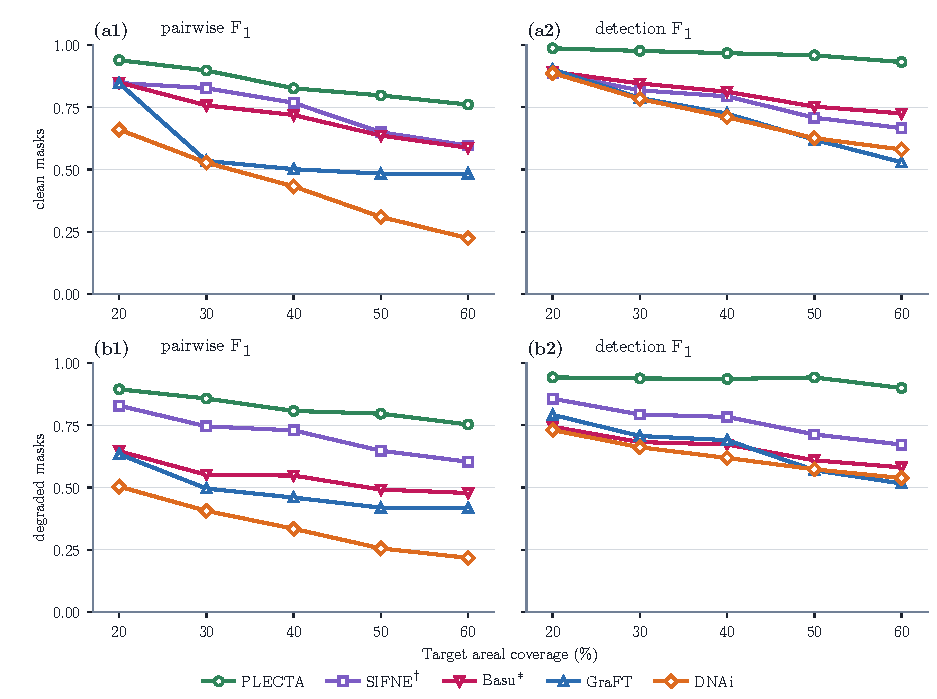
\includegraphics[width=\linewidth]{figures/fig_metric_panels.pdf}
  \caption{Five methods on identical masks, by coverage stratum. Rows: the
    undegraded axis, panels \textbf{(a)} and \textbf{(b)}, above the
    degraded one, panels \textbf{(c)} and \textbf{(d)}. Columns: pairwise
    \Fone{}, which counts pairs of fragments, and detection \Fone{} at IoU
    \PlectaDetectionIoU{} with a
    \PlectaPlacementTolerance{}\,px tolerance, which counts objects
    (Section~\ref{sec:mm-metrics}). The two disagree where a method
    fragments, since only the first is quadratic in fragmentation. Crossing
    Fidelity is in Table~\ref{tab:plecta-comparators}. Means of ten scenes.
    $^{*}$\,our reimplementation; none was found.}
  \label{fig:metric-panels}
\end{figure}

Under these comparator-favouring settings, the ranking of
Table~\ref{tab:plecta-comparators} remained constant across density levels
and mask conditions (Figure~\ref{fig:metric-panels}). SIFNE is the
strongest of them, so the margin is measured against a method configured for
this data rather than against an unsuitable default. Two entries qualify that ordering. The first is
DNAi, whose deficit is a limitation of domain and density rather than a
general ranking: it is built for DNA-fibre micrographs, which are sparse, and
where the network is sparse and the axis clean it recovers
\PlectaDNAiCleanSparseFOne{} at 20\% coverage. The second is
\citet{basu2015extraction}, the closest structural relative PLECTA's junction
matching has in that it too optimises over a neighbourhood and penalises
joins by curvature. It stands second only to PLECTA on Crossing Fidelity while its
pairwise \Fone{} is substantially below both released methods, so the curvature-priced
matching is effective at the junctions, and the deficit arises in the
stages around that decision. That is why the unmatched-arm penalty of
Section~\ref{sec:mm-plecta} is claimed as part of a combination rather than
on its own. \suppcomparators{} gives both in full.

\textbf{Each method in its own regime.} That ordering is drawn from one
generator, so it was tested in the regimes the two released methods were built
for. On GraFT's own generator, run unmodified at its published settings over
\PlectaRegimeSceneCount{} scenes in \PlectaRegimeStratumCount{} density
strata, PLECTA achieved the highest \Fone{} at every density and no rank
reversals occurred, including inside the range GraFT itself published, and
the field-standard measures order the three identically. Overall it
achieved
\Fone{}=\PlectaRegimeOverallPlectaFOne{} there, against
\PlectaRegimeOverallGraFTFOne{} for GraFT on its own scenes and
\PlectaRegimeOverallDNAiFOne{} for DNAi. SIFNE released no generator, so the sparse cobweb
topology its paper validates against was rebuilt here from that description;
on that reconstruction the two methods are level in the regime the SIFNE
publication addresses,
\PlectaSifneOwnSparsePlectaFOne{} against \PlectaSifneOwnSparseSifneFOne{},
and separate only slightly at the denser end. That places the difference in
the degree of crossing entanglement rather than in the total strand content
of the frame,
though a topology we rebuilt is weaker evidence than a generator its authors
released. \suppcomparators{} gives both density series in full.


\textbf{Cost.} The methods differ in computational cost as well as in
accuracy. Per-scene cost was measured warm, single-threaded and pinned to
one core, timing each method's own computation only
(Table~\ref{tab:plecta-comparators}). These
are independently optimised codebases, so absolute times measure
implementation as much as algorithm.

\textbf{On real imaging.} The two comparators that read a binary axis were run
over the \PlectaRealFieldCountLower{} annotated fields as well, on the
manual-derived masks of Section~\ref{sec:res-real} and through the same
scoring pipeline as PLECTA on those fields.
Averaged over the \PlectaRealFieldCountLower{}, PLECTA achieved
\Fone{}=\PlectaRealManualFOneMean{}, against \PlectaRealSifneFOneMean{} for
SIFNE and \PlectaRealBasuFOneMean{} for Basu, and the highest value on every
measure reported. The ordering established on synthetic scenes therefore holds on
masks read off real micrographs.

The margin is narrower than on the synthetic scenes, which likely reflects
the quality of the manually derived axes: a skeleton of a hand annotation is
unbroken, thin and placed where a person judged the strand to be, so it
contains few of the fragmentation and displacement artefacts responsible for
the differences observed in the synthetic evaluation.
